\chapter{Gennemgang af detektionsmetoder}\label{sec:detmet}
I denne sektion vil, der udføres en gennemgang af forskellige detektionsmetoder. Visse metoder er udvalgt, da de også er blevet implementeret og afprøvet på markbilleder. <I dette afsnit vil der også gives eksempler på udvalge metodernes indvirkning på billeder> 

\section{Moravec}\label{sec:moravec}
Moravec's hjørne detektor, beskrevet i \cite{moravec}, er en af de første hjørnedetektorer, og definere et hjørne som værende et område, hvor der opstår store intensitetsskift. <correlation>. Moravec anvender denne definition til at opnå en matematisk formulering af hjørner ved at bygge videre på notationen om et kvadratisk vindue, omliggende det undersøgte punkt, diskuteret i \ref{subsec:corner}, typisk i størrelser af 3x3, 5x5 eller 7x7 pixel regioner. Sammenlignes to vinduer, hvor begge portrættere det samme objekt, vil intensitetsvariationen imellem disse vinduer være 0.
De interessante punkter findes da når auto-korrelationen imellem de forskudte billeder er stor. Forskydningsvinduet kan derved bruges til at detektere hjørner, ved at tage et pixel område omkring et punkt, forskyde dette vindue med 1 pixel i alle principielle retninger (horisontalt, vertikalt og diagonalt) og udregne intensitetsvariationen. Denne variation kan beskrives med en vægtet funktion over vinduet  \emph{(WSSD: weighted summed square difference)}, der udregner forskellen på vinduerne:
\begin{equation}
E(u,v)= \sum w(x,y)[I(x,y)-I(x+u,y+v)]^2     
\end{equation}
hvor $(u,v)$ er forskydningsvektoren, der bevæger sig mellem intervallet [-1,1], og summere over alle \textit{i} pixels i regionen . Den mindste forskel: $C(x,y)=min(E(u,v))$ i de otte skift, definere punktets \textit{"hjørnestyrke"}. Den mindste forskel tages da et punkt, der er lokaliseret langs en kant, resultere i et stort intensitetsskifte når kanten krydses, men lille skift ved bevægelse langs kanten. Der er ikke et specifikt minimum af, der definere et hjørne. Der anvendes derfor en grænseværdi for hvornår der opstår et hjørne. Figur \ref{fig:moravec} illustrere en udregning af \textit{WSSD} af et diagonalt skift på en isoleret sort pixel (med en intensitet på 0) på en hvid baggrund (med en intensitet på 255) og på et idealt hjørne. Det røde vindue indikere det originale vindue og det blå vindue indikere  vinduet forskudt med vektoren $u = (1,1)$. 
\begin{figure}[H]
    \centering
    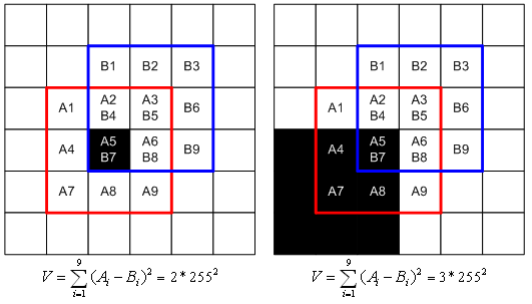
\includegraphics[width=0.45\textwidth]{fig/25.png}
     \vspace{-1em}
    \begin{center}    
       \caption{\textcolor{gray}{\footnotesize \textit{ WSSD udregninger for intensitetsvariationer imellem forskudte vindue. }}}
    \label{fig:moravec}
     \end{center}
     \vspace{-2.5em}
  \end{figure} \noindent
Moravec lider af følgende række problemer pga. dens simplicitet. 
\begin{itemize}
\item{ Der undersøges kun et diskret sæt af pixelskift (i hver principiel orientering) og resultatet er derfor anisotropisk. Undersøges en kant, der ikke er horisontal, vertikal eller diagonal ift. punktet vil den mindste intensitetsvariation være stor, og derved kan punktet fejlagtigt detekteres som et hjørne. Dette medfører også at detektionen ikke er rotationsinvariant.}
\item{Det skiftende vindue er rektangulær og binært, metoden er derfor meget følsom overfor støj i billedet.}
\item{Detektoren finder punkter lokaliseret på kanter. I sektion \ref{subsec:kant} defineres en kant som værende et pludseligt skift i intensiteten i en given retning. Små deformationer i kanterne som støj, vil resultere i at den mindste intensitetsvariation vil være relativt stor, og derfor detektere punktet som værende et interessepunkt.}
\end{itemize}
% <evt konklusion>
% <måske billeder download cornerdetection.pdf>
\subsection*{Algoritme:}
\begin{enumerate}
\item{For hvert pixel i billedet, udregnes auto-korrelationen imellem skift af $(u,v) \in [-1,0,1]$. udregnet ved \textit{WSSD} }
\item{\textit{"Hjørnestyrken"} udregnes for hvert pixel ved at finde $C(x,y)=min(E(u,v))$ }
\item{ En grænseværdi sættes sættes for $C(x,y)$}
\item{lokale ekstremaer identificeres. }
\end{enumerate}
\subsection*{Eksempler?}
\subsection*{Konklusion}
Moravec er som nævnt en simpel algoritme, med mange udfordringer, der gør at den ikke bruges som en repeterbar detektor. Detektoren er i dag ikke i sig selv relevant, som den var da den blev udgivet, men bygges videre på i andre detektorer, f.eks. \textit{"Harris"} beskrevet i sektion, \ref{sec:harris} som direkte tilgår de nævne problemstillinger med Moravec.
\section{Harris}\label{sec:harris}
"Harris" hjørnedetektor er en metode introduceret af Chris Harris og Mike Stephens i 1988 \cite{harris}. Metoden refereres til som "Harris hjørnedetektor", men er også kendt som "Plessy". Metoden tager fat i Moravec's detektor og bygger videre på denne ved at adressere metodens begrænsninger, beskrevet i sektion \ref{sec:moravec}.
\begin{enumerate}
\item{ \textit{Anisotropisk respons:} Harris og Stephens har udvidet Moravecs udregning af auto-korrelation til at måle intensitetsvariationer i alle retninger. Auto korrelationen mellem skiftende vinduer kan approksimeres ved at udvide funktionen, ved en \textit{"Taylor udvidelse"} af 2 orden:
\begin{subequations}
\begin{align}
E(u,v) = & \sum w(x,y)[I(x+u),(y+v)-I(x,y)]^2 \\
\approx & \sum w(x,y)[I(x,y)+u I_x+v I_y-I(x,y)]^2 \\
= & \sum w(x,y)I(x,y)u^2 I_x^2+2uv I_x I_y + v^2 I_y^2 \label{last}
\end{align}
\end{subequations}
Ovenstående \eqref{last} kan omskrives til en overskuelig matrix operation:
\begin{equation}
E(u,v) \approx
\begin{bmatrix}
        u & v
     \end{bmatrix}
M
\begin{bmatrix}
        u \\
        v
     \end{bmatrix}
\end{equation} 
Hvor M er auto-korrelations matricen (også kaldt struktur-tensor), der består af horisontale og vertikale afledte af billedet:
\begin{equation}
M =  \sum w(x,y)
\begin{bmatrix}
I_x^2 & I_xI_y \\
I_xI_y & I_y^2
\label{M}
\end{bmatrix}
\end{equation}
Billedets afledte i x og y aksen findes ved at udføre en diskret differentiering af billedet, hvilket kan opnås
 ved at folde billedet, med henholdsvis $[-1 \hspace{0.1cm} 0 \hspace{0.1cm} 1]$ og $[-1 \hspace{0.1cm} 0 \hspace{0.1cm} 1]^T$. }
\item{\textit{Støj sensitiv:} Harris detektoren anvender et Gaussisk vindue omkring det undersøgte pixel område. Dette tilføjer en vægt i form af en cirkel omkring punktet. Det Gaussiske vindue anvendes til at fjerne støj fra billedet, da differentiering er følsom overfor dette.}
\item{\textit{Højt kant respons} Struktur-tensoren 'M' opskrevet i \eqref{M} indeholder de differentieret retninger i et givet punkt og derved en beskrivelse af billedets geometriske struktur, i et punkt (x,y). Egenværdierne for denne matrix, vil være proportionale med den principielle krumning i billedets flade og er derfor interessant ift. at finde hjørne. Egenværdierne vil være proportionale med de forskellige steder vinduet kan placeres:
\begin{enumerate}
\item{ \textit{Homogen flade.} Billede intensiteten er konstant. Begge egenværdier vil være små og der vil ikke være nogen krumning i billedet.}
\item{\textit{Kant.} For punkter placeret på en kant, vil der være en stor krumning på tværs af kanten, men ingen når kanten følges. Derfor vil én egenværdi være stor, mens den anden vil være lille}
\item{\textit{Hjørne.} Et punkt placeret på et hjørne, vil have en stor kurve, i hver retning og derved bestå af to store egenværdier.}
\end{enumerate}
Det ønskes derfor, for at identificere hjørner, at begge egenværdier for M er store. Egenværdierne kan defineres udefra determinanten og sporet af M:
\begin{subequations}
\begin{align}
\textbf{det}M & = \lambda_1 \lambda_2 \\
\textbf{trace}M & = \lambda_1+\lambda_2
\end{align}
\end{subequations}
Harris og Stephens foreslår følgende måde at definere "hjørnestyrken":
\begin{equation}
R = \textbf{det}M-k(\textbf{trace}M)^2
\end{equation}
hvor \textit{k} er en empirisk defineret konstant mellem $0.04-0.06$. I figur \ref{fig:egen} ses sammenhængen mellem værdien 'R', egenværdierne og hvordan de korrespondere med hjørner,kanter og homogene område, igen kan det ses at for et "stærkt" hjørne ønskes to store egenværdier.

\begin{figure}[H]
    \centering
    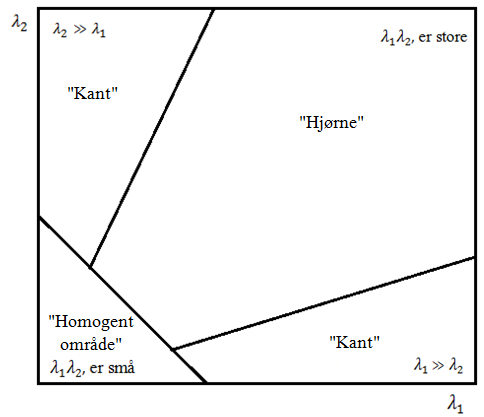
\includegraphics[width=0.45\textwidth]{fig/26.png}
     \vspace{-1em}
    \begin{center}    
       \caption{\textcolor{gray}{\footnotesize \textit{ Opdeling af egenværdi rummet til specifikke regioner. }}}
    \label{fig:egen}
     \end{center}
     \vspace{-2.5em}
  \end{figure} \noindent
Ved værdien for R, kan det defineres om et punkt er lokaliseret på et hjørne. De interessante hjørne, er hvor der opstår en stor "hjørnestyrke", hvilket kan findes ved at sætte en grænseværdi, der definere et hjørne.
 }
\end{enumerate}
\subsection*{Algoritme}
\begin{enumerate}
\item{ For hvert pixel i billedet (x,y), udregn struktur tensoren: $$ M = \begin{bmatrix}
I_x^2 & I_xI_y \\
I_xI_y & I_y^2
\end{bmatrix} $$hvor $ I_x^2 = (\dfrac{\partial I}{\partial x})^2 \ast w$, og w er et Gaussisk vindue.}
\item{ Konstruer et billede bestående af hjørnestyrken 'R' udregnet ved $$ R = \textbf{det}M-k(\textbf{trace}M)^2 $$  }
\item{ Opstil en grænseværdi for billedet bestående af 'hjørnestyrken'}
\item{ Lokaliser lokale ekstremaer }
\end{enumerate}
\subsection*{Konklusion}
Metoden anvendes som en repeterbar detektor og bruges i høj grad i dag. Detektoren er rotationsinvariant pga. dens brug af egenværdier, men er ifølge \cite{eval} stadig delvis anisotropisk, hvilket skyldes differentierings filtrene der kun bruges i x og y retningen. Mikolajczyk og Schmid \cite{eval} konkludere at detektoren er særlig følsom over for rotation omkring 45 grader. De konkludere også at detektorens repeterbarhed falder drastisk ved skalaændringer.
% måske begræsninger istedet
\subsection{Detektion}
SIFT gør brug af en metode kaldt Difference of Gaussian (DoG), til at finde interessepunkter. DoG er en skala-invariant blob detektor, og er en approksimation til en skalanormaliseret Laplacian of Gaussian (LoG). DoG kan udregnes, ved en subtraktion af et nærliggende skalabillede, separeret af en konstant $k$, hvor $G$ er et Gaussisk filter.
\begin{equation}
\begin{split}
DoG(x,y,\sigma) &= (G(x,y,k\sigma)-(G(x,y,\sigma))\ast I(x,y) \\
           &= L(x,y,k \sigma)-L(x,y,\sigma)
\end{split}
\label{dog}
\end{equation}
Den skalanormaliseret Laplacian of Gaussian kan opstilles som:
\begin{equation}
\begin{split}
LoG(x,y,\sigma)&=\sigma^2\nabla^2L(x,y,\sigma) \\
&= \sigma^2(L_{xx}+L{yy})
\end{split}
\end{equation}
Lowe relatere approksimeringen af DoG til LoG, ved diffusions ligningen:
\begin{equation}
\dfrac{\partial L}{\partial \sigma} = \sigma \nabla^2L
\label{heat}
\end{equation}
Ligning \eqref{heat} kan approksimeres til:
\begin{equation}
\sigma \nabla^2L \approx \frac{G(x,y,k\sigma) - G(x,y,\sigma)}{k\sigma-\sigma}
\label{omskriv}
\end{equation}
Omskrivning af ligning \eqref{omskriv} giver:
\begin{equation}
\begin{split}
(k\sigma-\sigma)\sigma\nabla^2L &\approx L(x,y,k\sigma)-L(x,y,\sigma) \\
(k-1)\sigma^2LoG &\approx DoG
\end{split}
\end{equation}
Metoden anvender et skalarum, der deles op i oktaver, hver bestående af skalabilleder. Skalabilleder opnås ved at folde billedet iterativt med et Gaussisk filter, af stigende sigma værdi, dvs. med en stigende grad af slørring. Sigma værdien for første skalabillede, for en given oktav $l$ er dobbelt så stor som forrige: $\texttt{Start} \sigma_l = 2 \cdot \texttt{Start} \sigma_{l-1}$. Sigma værdien for et nærliggende skalabillede på samme oktav, opnås ved at multiplicere sigma værdien med en konstant $k$, dvs. $\sigma_n = \sigma_{n-1} \cdot k$. I den udførte implementering er $k=\sqrt{2}$, hvor den første sigma værdi er $1.6$. Lowe anbefaler at bruge fire oktaver, hver med syv skalabilleder. I denne implementering er der brugt fire oktaver, med fem skalabilleder per. oktav, hvilket har vist sig, at give brugbare resultater. Metoden anvender en skalapyramide og billedet reduceres derfor, for hver oktav, med halv størrelse, ift. forrige oktav. \\ 
Når skalarummet er oprettet skal DoG billederne produceres, hvilket er illustreret i figur \ref{fig:difference}(a), hvor naboliggende skalabilleder i samme oktav subtraheres. \begin{figure}[H]
    \centering
    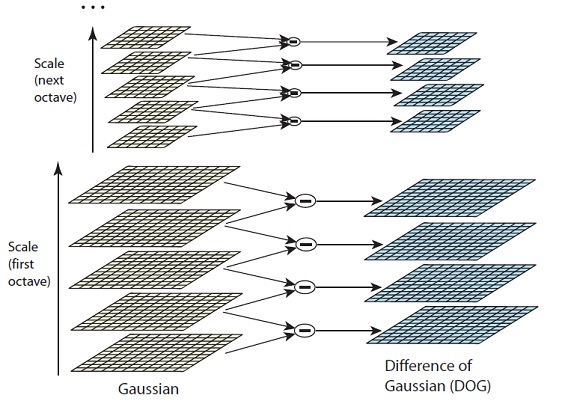
\includegraphics[width=0.90\textwidth]{fig/30.png}
     \vspace{-1em}
    \begin{center}    
       \caption{\textcolor{gray}{\footnotesize \textit{(a) Nærliggende skalabilleder for hver oktav trækkes fra og producere DoG billederne. (b) I DoG billederne udvælges ekstremaer blandt 27 nabo pixels.}}}
    \label{fig:difference}
     \end{center}
     \vspace{-2.5em}
  \end{figure} \noindent
LoG svarer til sporret af hessian matricen som angiver summen af hessian matricens egenværdier: $\nabla^2 L=\bold{tr}( \mathcal{H} )=\lambda_1+\lambda_2$. Hessian matricens egenværdier beskriver den principielle krumning i og omkring et punkt og kan derfor bruges til at udvælge forekomster af blobs. Der vil opstå et maksima når $\nabla^2 L<0$, da egenværdierne begge vil være negative og et minima når $\nabla^2 L > 0$ da egenværdierne vil være positive. Der ønskes derved at identificere ekstremaer i DoG billederne, da de vil angive forekomster af blobs. For hver pixel, sammenlignes et $3\times3\times3$ område, som vist figur \ref{fig:difference} (b). Hver pixel bliver sammenlignet med dens $8+9+9=26$ naboer i de omkringliggende DoG billeder. Et punkt udvælges som værende et ekstrema, hvis det er det største/mindste iblandt dens 26 naboer.
\\
\\
Når lokale ekstremaer er udvalgt fravælges dårligt lokaliserede punkter, f.eks. ekstremaer med lav kontrast, men også punkter, hvor ekstremaer ligger imellem pixels. Ligeledes bliver punkters placering fundet, med subpixel nøjagtighed. Dette gøres, ved non-maximal suppression, som foreslået af Lowe \cite{nonmaximalsuppression}:
\begin{equation}
D(x)=D+\dfrac{\partial D^T}{\partial x}x\dfrac{1}{2}x^T\dfrac{\partial^2D}{\partial x^2}x
\label{nonmax}
\end{equation}
Ovenstående kan forstås om en Taylor udvidelse af punket D.
Lokationen af ekstremaet $\hat{x}$ findes ved at tage den afledte af den ovenstående funktion ift. $x$ og sætte den til 0:
\begin{equation}
\hat{x}= \dfrac{\partial^2 D^{-1}}{\partial x^2}\dfrac{\partial D}{\partial x}
\label{xhat}
\end{equation}
I denne implementering er Non-maximal surpression anvendt anderledes ift. den anvendt i SIFT: Lowe foreslår, at hvis et punkt er et ekstrema, som udregnet ved ligning \ref{nonmax} og $\hat{x} > 0.5$ i en retning, skal ligning \eqref{nonmax} udregnes omkring det nye punkt og dette gentages, indtil $\hat{x} < 0.5$, eller indtil udregning er udført et max antal gange.
\\
I denne implementering bliver et punkt fjernet, hvis $\hat{x} > 0.5$ i en given retning, da dette kun vil øge antallet af interessepunkter, hvilket er vurderet til ikke at være nødvendigt, da der i forvejen lokaliseres et stort antal punkter. Det vil ligeledes øge kompleksiteten af applikationen.
\\
Punkter med lav kontrast fjernes, ved at sætte grænseværdi, for $D(\hat{x})$:
\begin{equation}
D(\hat{x})=D+\dfrac{1}{2}\dfrac{\partial D^T}{\partial x}\hat{x}
\label{dxhat}
\end{equation}
Lowe foreslår at værdier af $D(\hat{x})$ under 0.03 fjernes. Metoden vil også have en positiv respons overfor kanter, derfor anvendes metoder lånt fra Harris og Stephens \cite{harris} til at fjerne disse. Hessian matricen opstilles som:
\begin{equation}
\mathcal{H} =
\begin{bmatrix}
D_{xx} & D{xy} \\
D{xy} & D{yy}
\end{bmatrix}
\end{equation}
En negativ determinant angiver et saddle-point og fjernes derved. For at fjerne punkter lokaliseret på en kant beskrives forholdet imellem hessian matricens egenværdier, ved følgende ligning, hvor $r$ angiver størrelsesforholdet imellem egenværdierne:
\begin{equation}
\dfrac{tr(\mathcal{H})^2}{Det(\mathcal{H})}<\dfrac{(r+1)^2}{r}
\label{rval}
\end{equation}
En grænseværdi $r$ kan opstilles for at fjerne punkter lokaliseret på en kant. Punkter der tilfredsstiller denne grænseværdi udvælges som interessepunkter.
\subsection{Algoritme}
\textbf{Input:} \\
\textbf{Output:}
\begin{enumerate}
\item{Konstruer skalarummet for de forskellige oktaver, ved iterativt at folde skalabilledet med en stigende værdi af $\sigma$: $$ L(x,y,\sigma)= G(x,y,\sigma) \ast I(x,y) $$
og halver størrelsen af billedet for hver oktav.}
\item{Udregn DOG billeder, ved at tage forskellen imellem skala billederne, som i ligning \eqref{dog}.}
\item{Lokaliser ekstremaer for hvert punkt i DOG billeder, ved at sammenligne punktet med dens 26 naboer som illustreret i figur \ref{fig:difference}.}
\item{Afvis punkter der ikke er lokaliseret på ekstremaer, og ekstremaer med lav kontrast som i ligning \eqref{xhat} og \eqref{dxhat}:
\begin{equation}
\begin{split}
\texttt{indikator} = 
\begin{cases}
\texttt{fjern}& \texttt{hvis } \hat{x}>0.5 \lor |D(\hat{x})|>0.03 \lor \bold{det} \mathcal{H}<0 , \\
\texttt{behold}& \texttt{ellers}. 
\end{cases}
\end{split}
\label{maxsurp}
\end{equation}
}
\item{Fjern punkter lokaliseret på en kant ved at opstille en grænseværdi $r$ og fjern punkter der ikke opfylder denne, som i ligning \eqref{rval}.}
\end{enumerate}